\documentclass[a4paper, 12pt]{article}

% Better font selection
\usepackage{fontspec}

% PDF hyperlinks
\usepackage{hyperref}

% Graphics
\usepackage{tikz}
\usetikzlibrary{positioning}

% Place figures exactly where they are needed
\usepackage{float}

% Unicode math symbols
\usepackage{unicode-math}
% Use a math font which has support for "\"
\setmathfont{Libertinus Math}

% Mathematical commands
\usepackage{amsmath}
\usepackage{amsthm}
\usepackage{mathtools}

% Set notation
\usepackage{braket}

% Support for commenting out blocks of LaTeX code
\usepackage{verbatim}

\theoremstyle{definition}
\newtheorem*{theorem}{Theorem}
\newtheorem*{corollary}{Corollary}
\newtheorem*{definition}{Definition}
\newtheorem*{lemma}{Lemma}

\newcommand{\naturals}{\symbb{N}}
\newcommand{\reals}{\symbb{R}}
\newcommand{\complex}{\symbb{C}}
\newcommand{\ball}{\symcal{B}}

\DeclarePairedDelimiter{\ceil}{\lceil}{\rceil}
\DeclarePairedDelimiter{\norm}{\lVert}{\rVert}

% Command to number only one line in a multi-line equation
% Based on https://tex.stackexchange.com/a/42728
\newcommand\numberthis{\addtocounter{equation}{1}\tag{\theequation}}

\title{Proof of the open mapping theorem}
\author{Gabriel Majeri}
\date{}

\begin{document}

\maketitle

\begin{theorem}[Open mapping]
Let \(X\) and \(Y\) be two \textbf{complete normed spaces} and \(\Lambda \colon X \to Y\) a \textbf{surjective} and \textbf{bounded} \textbf{linear transformation}. Denote with \(U \subset X\) and \(V \subset Y\) the corresponding open unit balls. Then there exists a \(\delta > 0\) such that
\[
    \Lambda(U) \supseteq \delta V
\]
where \(\delta V = \Set{ \delta v \mid v \in V }\) is the open ball of radius \(\delta\) centered at \(0 \in Y\).
\end{theorem}

This is a graphical representation of the statement of the theorem:
\begin{figure}[H]
    \centering

    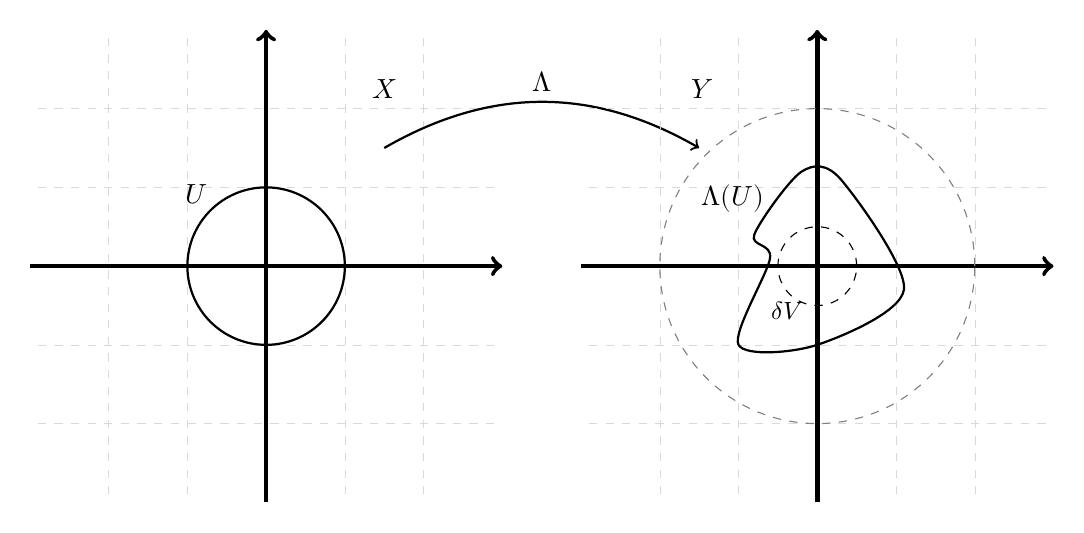
\begin{tikzpicture}
        \draw (1.5,2.25) node {\(X\)};
        \draw[help lines, color=gray!30, dashed] (-2.9,-2.9) grid (2.9,2.9);
        \draw[->,ultra thick] (-3,0)--(3,0);
        \draw[->,ultra thick] (0,-3)--(0,3);

        \draw[thick] (0,0) circle (1) node (U) {};
        \node[above left = 0.75 of U] {\(U\)};

        \draw[->, thick] (1.5, 1.5) to [out=30,in=150] node[above] {\(\Lambda\)} ++(4, 0);

        \begin{scope}[shift={(7, 0)}]
            \draw (-1.5,2.25) node {\(Y\)};
            \draw[help lines, color=gray!30, dashed] (-2.9,-2.9) grid (2.9,2.9);
            \draw[->,ultra thick] (-3,0)--(3,0);
            \draw[->,ultra thick] (0,-3)--(0,3);

            \draw [thick] node (LambdaU) {} plot [smooth cycle] coordinates {(-0.6,0.1) (-0.8,0.4) (-0.2,1.2) (0.3,1.1) (1.1,-0.3) (0,-1) (-1, -1)};
            \node[above left = 0.6 of LambdaU] {\(\Lambda(U)\)};

            \draw[dashed] (0,0) circle (0.5) node (DeltaV) {};
            \node[below left = 0.2 and 0 of DeltaV] {\small \(\delta V\)};
            \draw[dashed, gray] (0,0) circle (2);
        \end{scope}
    \end{tikzpicture}
\end{figure}

Since \(\Lambda\) is bounded, we are certain that \(\Lambda(U)\) is contained within some multiple of the open unit ball \(V\) (the large dashed gray circle in the figure). If the two spaces are complete and \(\Lambda\) is surjective, the theorem states that we can also fit some multiple of the open unit ball \emph{within} \(\Lambda(U)\) (the smaller dashed circle labeled with \(\delta V\) in the figure).

If we replace \(U\) in the hypothesis with some other open ball \(B\) of radius \(r\) and center \(c\), through linearity we get that \(\Lambda(B)\) contains an open neighborhood of \(\Lambda(c)\). Hence, \(\Lambda\) maps open sets to open sets, which makes it an open map. This is why the result is also known as the \textbf{open mapping theorem}.

\begin{proof}
First, we will show that we can fit \emph{an} open ball (of some center and radius) within \emph{some scaled multiple} of \(\Lambda(U)\).

Let \(y \in Y\). Since \(\Lambda\) is surjective, there exists some \(x \in X\) such that \(\Lambda(x) = y\). Let \(k\) be the smallest integer such that \(k > \norm{x}\). Then, by the way we've defined \(k\) we have \(x \in kU\) (the unit ball enlarged \(k\) times), hence \(y \in \Lambda(kU)\).

Since \(y\) was arbitrary, this shows that
\begin{equation} \label{decomposition_of_y}
    Y = \bigcup_{k = 1}^{\infty} \Lambda (kU)
\end{equation}
which is depicted graphically in the figure below (each contour represents the boundary of some \(\Lambda(kU)\)).

\begin{figure}[h!]
    \centering
    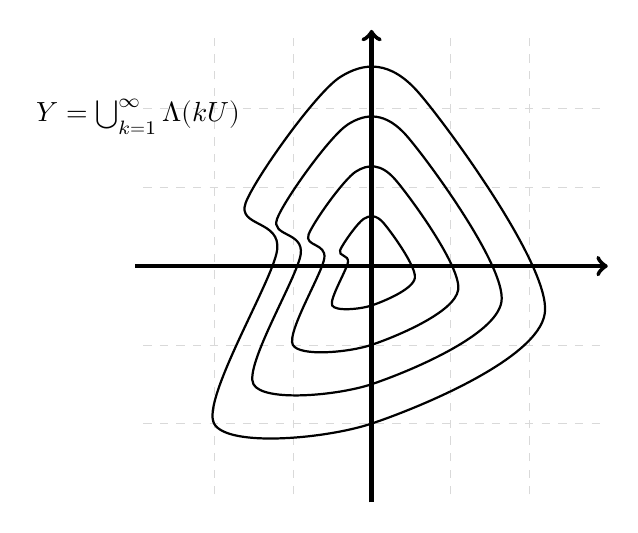
\begin{tikzpicture}
        \draw[help lines, color=gray!30, dashed] (-2.9,-2.9) grid (2.9,2.9);
        \draw[->,ultra thick] (-3,0)--(3,0);
        \draw[->,ultra thick] (0,-3)--(0,3);

        \draw [thick, scale=0.5] node (LambdaU) {} plot [smooth cycle] coordinates {(-0.6,0.1) (-0.8,0.4) (-0.2,1.2) (0.3,1.1) (1.1,-0.3) (0,-1) (-1, -1)};

        \draw [thick, scale=1] node (2LambdaU) {} plot [smooth cycle] coordinates {(-0.6,0.1) (-0.8,0.4) (-0.2,1.2) (0.3,1.1) (1.1,-0.3) (0,-1) (-1, -1)};

        \draw [thick, scale=1.5] node (3LambdaU) {} plot [smooth cycle] coordinates {(-0.6,0.1) (-0.8,0.4) (-0.2,1.2) (0.3,1.1) (1.1,-0.3) (0,-1) (-1, -1)};

        \draw [thick, scale=2] node (4LambdaU) {} plot [smooth cycle] coordinates {(-0.6,0.1) (-0.8,0.4) (-0.2,1.2) (0.3,1.1) (1.1,-0.3) (0,-1) (-1, -1)};

        \node[above left = 2 of 4LambdaU] {\(Y = \bigcup_{k = 1}^{\infty} \Lambda(kU)\)};
    \end{tikzpicture}
\end{figure}

Now, we will need to use another result known as the Baire category theorem.
\begin{theorem}[Baire]
If a complete metric space \(X\) is written as the union of a \textbf{countable} family of \textbf{closed} sets, then at least one of them has \textbf{non-empty interior}.
\end{theorem}

If we take the closure on both sides in equation \ref{decomposition_of_y} and use the fact that \(Y\) is complete, we have
\[
    Y = \bigcup_{k=1}^{\infty} \overline{\Lambda(kU)}
\]

Applying Baire's theorem, we conclude that there exists at least one \(k' \in \naturals^*\) such that
\[
    \overline{\Lambda(k' U)}^{\, \symrm{o}} \neq \emptyset
\]

By the definition of the interior, there exists at least one open set \(V\) such that \(V \subset \overline{\Lambda(k'U)}\). Since \(V\) is open in a normed space, it means that we can fit an open ball \(\ball_r (c)\) inside \(V\), for some \(r \in \reals^*_+\) and \(c \in V\).

\begin{figure}[!ht]
    \centering
    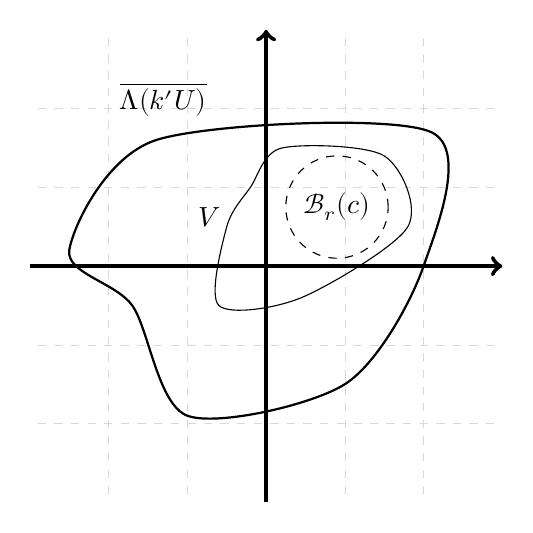
\begin{tikzpicture}
        \draw[help lines, color=gray!30, dashed] (-2.9,-2.9) grid (2.9,2.9);
        \draw[->,ultra thick] (-3,0)--(3,0);
        \draw[->,ultra thick] (0,-3)--(0,3);

        \draw [thick] node (LambdaKPrimeU) {} plot [smooth cycle] coordinates {(-2.5, 0.2) (-1.4,1.6) (2.1,1.7) (2,0) (1,-1.5) (-1,-1.9) (-1.7, -0.5)};
        \node[above left = 1.65 and 0.5 of LambdaKPrimeU] {\(\overline{\Lambda(k'U)}\)};

        \draw node (V) {} plot [smooth cycle] coordinates {(-0.2, 1) (0.2, 1.5) (1.5, 1.4) (1.8, 0.5) (0.45, -0.4) (-0.6, -0.5) (-0.5, 0.5)};
        \node[above left = 0.25 and 0.4 of V] {\(V\)};

        \draw[dashed] (0.9,0.75) circle (0.65) node {\(\ball_r(c)\)};
    \end{tikzpicture}
\end{figure}

Before we can proceed with the proof of the theorem, we will introduce the following lemma:
\begin{lemma}
    Let \(\delta \coloneqq \frac{r}{2k'}\) For all \(y \in Y\) and \(\epsilon > 0\), there exists an \(x \in X\) with
    \begin{equation} \label{definition_of_x}
        \norm{x} < \delta^{-1} \norm{y}
        \text{ and }
        \norm{y - \Lambda(x)} < \epsilon
    \end{equation}
    In words: for any vector of \(Y\) we can find a corresponding vector of \(X\) with a bound on its norm, such that its image through \(\Lambda\) differs from the target vector by at most \(\epsilon\).
\end{lemma}
\begin{proof}
We will prove the lemma for vectors in \(Y\) with norm smaller than \(r\), and then use linearity to extend the result to vectors of all magnitudes.

Let \(y \in Y\) be a vector with \(\norm{y} < r\). Then:
\begin{gather*}
    \norm{y} < r \\
    \implies \norm{c - c + y} < r \\
    \implies d(c, c + y) < r \\
    \implies c + y \in \ball_r (c)
\end{gather*}

Since \(c \in V \subset \overline{\Lambda(k'U)}\) and \(c + y \in \ball_r (c) \subset V \subset \overline{\Lambda(k'U)}\), by the definition of the closure of a set we can find sequences \((y'_n)_{n \in \naturals} \subset \Lambda(k'U)\) and \((y''_n)_{n \in \naturals} \subset \Lambda(k'U)\) such that
\begin{align*}
    y'_n &\rightarrow c \\
    y''_n &\rightarrow c + y
\end{align*}

By the surjectivity of \(\Lambda\), we can form two corresponding sequences \((x'_n)_{n \in \naturals} \subset k'U\), \((x''_n)_{n \in \naturals} \subset k'U\) such that
\begin{align*}
    \Lambda(x'_n) &= y'_n \\
    \Lambda(x''_n) &= y''_n
\end{align*}

Denote \(x_n = x''_n - x'_n\). Using the linearity of \(\Lambda\) we have that
\begin{gather*}
    \Lambda(x_n) = \Lambda(x''_n - x'_n) = \Lambda(x''_n) - \Lambda(x'_n) = y''_n - y'_n
\end{gather*}

The difference of two convergent sequences converges to the limit of the differences, therefore
\[
    \lim_{n \to \infty} \Lambda(x_n) = \lim_{n \to \infty} \left(y''_n - y'_n\right) = y
\]
Rewriting this using the definition of the limit, we have that \(\forall \epsilon > 0\), \(\exists N_\epsilon \in \naturals\) such that
\begin{equation}  \label{norm_of_y_minus_lambda_xn}
    \norm{y - \Lambda(x_{N_\epsilon})} < \epsilon
\end{equation}

The distance between any two points \(x'_n\) and \(x''_n\) of the open ball \(k'U = \ball_{k'} (0)\) is at most its diameter, therefore
\begin{equation} \label{norm_of_xn}
    \norm{x_n} = \norm{x''_n - x'_n} < 2k'
\end{equation}

Combining \ref{norm_of_y_minus_lambda_xn} with \ref{norm_of_xn}, we obtain an \(x \coloneqq x_{N_\epsilon}\) which satisfies the inequalities in the lemma.

Linearity allows us to expand the above result to all of \(Y\). If \(\norm{y'} \geq r\), then we can find a \(y\) with \(\norm{y} < r\) such that \(y' = \lambda y\) for some \(\lambda > 0\). Define \(\widetilde{x}'_n = \lambda \widetilde{x}_n\), and all the statements still hold.
\end{proof}

Now we are ready to prove the theorem. The idea is to inductively build a convergent sequence of vectors \(x_n\) such that \(\Lambda(x_1 + \dots + x_n) \to y\), as suggested in the following figure:
\begin{figure}[H]
    \centering
    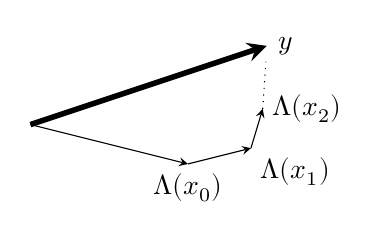
\begin{tikzpicture}
        \draw[line width=2pt, -stealth] (0, 0) -- (3, 1) node[anchor=west] {\(y\)};

        \draw[-stealth] (0, 0) -- (2, -0.5) node[anchor=north] {\(\Lambda(x_0)\)};
        \draw[-stealth] (2, -0.5) -- (2.8, -0.3) node[anchor=north west] {\(\Lambda(x_1)\)};
        \draw[-stealth] (2.8, -0.3) -- (2.95, 0.2) node[anchor=west] {\(\Lambda(x_2)\)};
        \draw[dotted] (2.95, 0.2) -- (2.99, 0.8);
    \end{tikzpicture}
\end{figure}

Let \(y \in \delta V\) and \(\eta > 0\). We apply the lemma (\ref{definition_of_x}) with \(\epsilon = \frac{1}{2} \delta \eta\) and obtain an \(x_0\) with the properties
\[
    \norm{x_0} < \delta^{-1} \norm{y} = \delta^{-1} \delta = 1
\]
and
\[
    \norm{y - \Lambda(x_0)} < \frac{1}{2} \delta \eta
\]
Applying the lemma again for \(y - \Lambda(x_0)\) and \(\epsilon = \frac{1}{4} \delta \eta\), we can obtain an \(x_1\) with
\[
    \norm{x_1} < \delta^{-1} \norm{y - \Lambda(x_0)} < \frac{1}{4} \eta
\]
and
\[
    \norm{y - \Lambda(x_0) - \Lambda(x_1)} = \norm{y - \Lambda(x_0 + x_1)} < \frac{1}{2} \delta \eta
\]

Define the sequence \((\overline{x_n})_{n \in \naturals} \subset X\) as
\[
    \overline{x_n} \coloneqq \sum_{i = 0}^{n} x_i
\]
so that we can write
\[
    \Lambda(x_0 + x_1 + \dots + x_n) = \Lambda(\overline{x_n})
\]

The induction hypothesis is that we already have some \(x_0, x_1, \dots, x_n\) with
\begin{gather*}
    \norm{x_n} < \frac{1}{2^n} \eta \\
    \norm{y - \Lambda(\overline{x_n})} < \frac{1}{2^{n + 1}} \delta\eta
\end{gather*}
We apply the lemma (\ref{definition_of_x}) to \(y - \Lambda(\overline{x_n})\) with \(\epsilon = \frac{1}{2^{n + 2}} \delta\) and we obtain an \(x_{n + 1}\) with
\begin{align*}
    \norm{x_{n + 1}} &< \delta^{-1} \norm{y - \Lambda(\overline{x_n})} \tag{from the lemma} \\
    &< \delta^{-1} \frac{1}{2^{n + 1}} \delta \eta \tag{by induction hypothesis} \\
    &= \frac{1}{2^{n + 1}} \eta \tag{reduce \(\delta\) with \(\delta^{-1}\)}
\end{align*}
and
\begin{align*}
    \norm{y - \Lambda(\overline{x_n}) - \Lambda(x_{n + 1})}  < \frac{1}{2^{n + 2}} \delta \eta \tag{from the lemma} \\
    \norm{y - \Lambda(x_1 + x_2 + \dots + x_n) - \Lambda(x_{n + 1})} < \frac{1}{2^{n + 2}} \delta \eta \tag{by the definition of \(\overline{x_n}\)} \\
    \norm{y - \Lambda(x_1 + x_2 + \dots + x_n + x_{n + 1})} < \frac{1}{2^{n + 2}} \delta \eta \tag{by linearity of \(\Lambda\)} \\
    \norm{y - \Lambda(\overline{x_{n + 1}})} < \frac{1}{2^{n + 2}} \delta \eta
\end{align*}
which is precisely what we had to show for the \(n + 1\) step of the induction.

We conclude that
\begin{gather}
    \label{upper_bound_on_xn}
    \norm{x_n} < \frac{1}{2^n} \eta \\
    \label{upper_bound_on_y_minus_lambda_xn}
    \norm{y - \Lambda(\overline{x_n})} < \frac{1}{2^{n + 1}} \delta \eta
\end{gather}
for all \(n \in \naturals\).

We remark that \(\norm{\overline{x_n} - \overline{x_{n - 1}}} = \norm{x_n}\), therefore from inequality \ref{upper_bound_on_xn} we get that \(\norm{\overline{x_n} - \overline{x_{n - 1}}} < \frac{1}{2^n} \eta\), i.e. the sequence \((\overline{x_n})\) is Cauchy. Because \(X\) is complete, it means \((\overline{x_n})\) is convergent to some point \(\overline{x} \in X\).

We will prove two facts about \(\overline{x}\):
\begin{itemize}
    \item \(\overline{x}\) is contained within the ball of radius \(1 + \eta\) centered at \(0 \in X\). Indeed, using the triangle inequality, we see that:
    \[
        \norm{\overline{x}}
        = \norm*{\lim_{n \to \infty} \sum_{i = 0}^{n} x_i}
        = \norm*{\sum_{i=0}^{\infty} x_i}
        \leq \sum_{i=0}^{\infty} \norm*{x_i}
        < \sum_{i=0}^{\infty} \frac{1}{2^i} \eta
        = 1 + \eta
    \]
    hence \(\overline{x} \in (1 + \eta) \, U\).

    \item \(\Lambda(\overline{x}) = y\). To show this, take the limit of inequality \ref{upper_bound_on_y_minus_lambda_xn}:
    \[
        \lim_{n\to\infty} \norm{y - \Lambda(\overline{x_{n+1}})} = 0
    \]
    and use the continuity of the norm and of \(\Lambda\) to conclude that \(y = \Lambda(\overline{x})\).
\end{itemize}

From these two facts we can conclude that \(y \in \Lambda((1 + \eta) \, U)\). We took \(y \in \delta V\) arbitrarily, hence
\[
    \delta V \subseteq \Lambda((1 + \eta) \, U)
\]
We can rewrite this using linearity:
\begin{gather*}
    \iff \delta V \subseteq (1 + \eta) \Lambda(U) \\
    \iff \frac{1}{1 + \eta} \, \delta V \subseteq \Lambda(U)
\end{gather*}
for all \(\eta > 0\).

By taking the union of \(\frac{1}{1 + \eta} \delta V\) over all \(\eta > 0\) we obtain
\[
    \delta V \subseteq \Lambda(U)
\]
\end{proof}

We will now prove an immediate consequence of the previous theorem:
\begin{theorem}[Bounded inverse]
Let \(X\) and \(Y\) be two \textbf{complete normed spaces} and \(\Lambda \colon X \to Y\) a \textbf{bijective} and \textbf{bounded} \textbf{linear transformation} between them. \\
Then there exists a \(\delta > 0\) such that
\[
    \norm{\Lambda(x)} \geq \delta \norm{x}, \forall x \in X
\]
and therefore \(\Lambda^{-1}\) is a \textbf{bounded} \textbf{linear transformation}.
\end{theorem}
\begin{proof}
Since \(\Lambda\) is bijective, we know that the inverse \(\Lambda^{-1} \colon Y \to X\) exists.

Furthermore, we can check that it is a linear transformation. We know \(\Lambda\) is linear, therefore
\[
    a \Lambda(u) + b \Lambda(v) = \Lambda(au + bv)
\]
for all \(a, b \in \complex\), \(u, v \in X\). Then, by applying \(\Lambda^{-1}\) to the equation we get
\[
    \Lambda^{-1} (a \Lambda(u) + b \Lambda(v)) = \Lambda^{-1}(\Lambda(au + bv)) = au + bv
\]
If we denote \(\Lambda(u)\) with \(u'\), \(\Lambda(v)\) with \(v'\), then \(u = \Lambda^{-1}(u')\) and \(v = \Lambda^{-1}(v')\). We have that
\[
    \Lambda^{-1} (a u' + b v') = a \Lambda^{-1} (u') + b \Lambda^{-1} (v')
\]
for all \(u', v' \in Y\), since \(\Lambda\) is surjective.

To prove that \(\Lambda^{-1}\) is bounded, by definition we need to show that there exists a \(\delta' > 0\) such that
\[
    \norm{\Lambda^{-1}(y)} \leq \delta' \norm{y}, \forall y \in Y
\]
Since \(\Lambda\) is bijective, by letting \(y = \Lambda(x)\) we obtain the equivalent statement:
\[
    \norm{x} \leq \delta' \norm{\Lambda(x)}, \forall x \in X
\]
Moving \(\delta'\) to the left, we get:
\[
    \delta'^{-1} \norm{x} \leq \norm{\Lambda(x)}, \forall x \in X
\]

Let \(\delta > 0\) be the constant we get for this hypothesis from the open mapping theorem. We know that every \(y \in Y\) with \(\norm{y} < \delta\) is the image \(\Lambda(x)\) of some \(x \in X\) with \(\norm{x} < 1\). But since \(\Lambda\) is bijective, this \(x\) is unique; there cannot be another \(x'\) (with norm possibly greater than \(1\)) such that \(\Lambda(x') = y\). So \(\norm{\Lambda(x)} < \delta \implies \norm{x} < 1\).

By negating this proposition, we obtain that when \(\norm{x} \geq 1\) we must have \(\norm{\Lambda(x)} \geq \delta\).

Setting \(\delta'^{-1} = \delta\), the condition above can be rewritten as:
\[
    \norm{\Lambda(x)} \geq \delta \norm{x}, \forall x \in X
\]
which is true based on the linearity of \(\Lambda\). Hence \(\Lambda^{-1}\) is a bounded linear map and \(\norm{\Lambda^{-1}} = \delta^{-1}\).
\end{proof}
\end{document}
